\section{Particles in an 1D Potential - 一维空间具有势能的粒子运动}
From the prevous section, we have the Hamiltonian of a particle in 1D continous space to be:
$$\hamiltonian = \frac{\opmtm^2}{2\mu} + V(\oppos)$$
Our goal now is to solve many Schr\"odinger's Equations with different $V(x)$. We primarily focus on using the time-independent Schr\"odinger's Equation related to the position wavefunction:
$$-\frac{\hbar^2}{2\mu}\pdv[2]{x} \psi(x, t) + V(x)\psi(x, t) = E \psi(x, t)$$

\subsection{Particle in a Box - 闭盒中的粒子}
We start with a special case, where the potential energy as a function of position is defined as follows:
$$V(x) = \begin{cases}
    0, & x \in [0, L] \\
    \infty, & \text{otherwise}
\end{cases}$$
The boundary conditions include:
\begin{quote}
    1. For $x$ outside the box, the potential energy is positive infinity, meaning the particle cannot be outside, as it has $0$ probability of being measured. This translates to:
    $$\forall t, \forall x \notin [0, L], \psi(x, t) = 0$$
    2. We want at least a continuous wavefunction, which means:
    $$\forall t, \psi(0, t) = \psi(L, t) = 0$$
\end{quote}
This thus gives us two parts:
$$\begin{cases}
    x \in [0, L]: & -\frac{\hbar^2}{2\mu}\pdv[2]{x} \psi(x, t) = E \psi(x, t) \\
    x \notin [0, L]: & -\frac{\hbar^2}{2\mu}\pdv[2]{x} \psi(x, t) + V(x)\psi(x, t) = E \psi(x, t)
\end{cases}$$
where in the second case, $V(x)\psi(x, t) = 0$. \\
We solve for $\psi(x)$ and $E$. It is claimed that for this equation, we have the wavefunction to be:
$$\psi_n(x) = \begin{cases}
    A\sin(k_n x), & x \in [0, L] \\
    0, & x \notin [0, L]
\end{cases}$$
and we solve the equation for $n = 1, 2, 3, \dots$ with
$$k_n = \frac{\pi n}{L}, E_n = \frac{\hbar^2 k_n^2}{2\mu} = \frac{\hbar^2 \pi^2 n^2}{2L^2 \mu} = E_1 \cdot n^2$$
These can be easily checked by substituting the relevant factors into the equation. More importantly, the normalization factor $A$ can be obtained by:
\begin{align*}
    \int_{0}^{L} \abs{\psi_n(x)}^2 \dd x &= 1 \\
    A &= \sqrt{\frac{2}{L}}
\end{align*}
For the time evolution, we can consider an arbitrary state like $\ket{\psi(0)} = \frac{1}{\sqrt{2}}(\ket{\psi_l} + \ket{\psi_m})$, and observe its time evolution to find out the wavefunction's evolution. \\
From this particle in a box calculation, we observe that:
\begin{quote}
    1. The energy spectrum and the solution to the Schr\"odinger's Equation is ``quantized'' (i.e. discrete, not continuous). An energy measurement ($\hamiltonian$ observable) can only give discrete outcomes like $E_1, E_2, \dots$. \\
    2. Formally, the quantization comes from the boundary condition where $\psi(0) = \psi(L) = 0$.
\end{quote}

\subsection{Continuity Conditions - 波函数连续性条件}
From the Schr\"odinger's equation, consider the part $-\frac{\hbar^2}{2\mu}\pdv[2]{x} \psi(x)$, we expect that $\psi \in C^2$, that is twice-differentiable and continuous. However, if we magnify at the boundary, depending on the potential chosen, a twice-differentiable and continuous wavefunction may be too much to ask for. Therefore, the \impt{minimum requirement} requires that $\abs{\psi(x)}^2$ to be a probability density. That is, the cumulative distribution:
$$\Prob{[x_1, x_2]}_\psi = \int_{x_1}^{x_2} \abs{\psi(x)}^2 \dd x$$
must be \impt{absolutely continuous}. For this, $\psi(x)$ must be \impt{continuous}. \\
Furthermore, if the \impt{potential energy is a constant} ($V(x) \in \R$), then the equation becomes:
$$\pdv[2]{x} \psi(x) = -\frac{2\mu}{\hbar^2}(E - V(x))\psi(x)$$
which by integrating both sides, we have
$$\pdv{x} \psi(x) = -\frac{2\mu}{\hbar^2} \int_{x_0}^{x_1} (E - V(x))\psi(x) \dd x$$
If $\psi$ is continuous, then we see its first derivative exists and is continuous due to the fact that \impt{the convolution of a real and continuous function is continuous}. \\
If the \impt{potential energy is continuous function} (i.e. a physical case), then we know the wavefunction $\psi \in C^2$.

\subsection{Bounded Interaction Zones in 1D - 一维空间的有限交互}
The general goal here is to solve the Schr\"odinger's Equation for the potential energy as a function of the position $V(x)$ in the form of:
$$V(x) = \begin{cases}
    V_L, & x \le x_L \\
    f(x), & x \in [x_L, x_R] \\
    V_R, & x \ge x_R
\end{cases}$$
The region $[x_L, x_R]$ is considered the ``interaction zone''. The idea is to solve the equation for each region independently and impose the continuity conditions that apply accordingly. \\
We first investigate the zones of constant $V(x)$ where for $x$ in these zones, $V(x) \equiv V_0$. We consider two cases:
\begin{quote}
    1. $E \ge V_0$: the equation becomes
    $$\pdv[2]{x} \psi(x) = -\frac{2\mu}{\hbar^2}(E - V_0)\psi(x)$$
    where we denote
    $$k = \sqrt{\frac{2\mu(E-V_0)}{\hbar^2}}$$
    so the equation ultimately becomes:
    $$\pdv[2]{x} \psi(x) = -k^2\psi(x)$$
    which gives us the general solution of
    $$\psi(x) = Ae^{\imag k x} + Be^{-\imag k x}$$
    where $A, B \in \C$ and they are determined by the continuity conditions. \\
    2. $E < V_0$: the equation becomes
    $$\pdv[2]{x} \psi(x) = \frac{2\mu}{\hbar^2}(V_0 - E)\psi(x)$$
    where we denote
    $$b = \sqrt{\frac{2\mu(V_0 - E)}{\hbar^2}}$$
    so the equation ultimately becomes:
    $$\pdv[2]{x} \psi(x) = b^2\psi(x)$$
    which gives us the general solution of
    $$\psi(x) = Ce^{b x} + De^{- b x}$$
\end{quote}
For the $E \ge V_0$ cases, we have the following notes:
\begin{quote}
    1. $\psi(x) = e^{\imag k x}$ is the position wavefunction for a particle travelling from left to right $(k > 0)$. This is demonstrated by looking at how the momentum operator acts on the wavefunction:
    \begin{align*}
        \opmtm \psi(x) &= -\imag \hbar \pdv{x}\psi(x) \\
        &= -\imag\hbar(\imag k e^{\imag k x}) 
        &= \hbar k \psi(x)
    \end{align*}
    We observe that $\psi(x)$ is an eigenfunction of $\opmtm$ with eigenvalue $\hbar k$. \\
    Thus, $\psi(x)$ is a position wavefunction in $\ket{p}$ with $p = \hbar k$. The corresponding momentum wavefunction is:
    \begin{align*}
        \tilde{\psi}(p) &= \frac{1}{\sqrt{2\pi\hbar}} \intR \exp(-\frac{\imag p x}{\hbar}) \exp(\imag k x) \dd x \\
        &= \frac{1}{\sqrt{2\pi\hbar}} \intR \exp(-\imag (p - \hbar k) y) \dd y, y = \frac{x}{\hbar} \\
        &= \delta(p - \hbar k)
    \end{align*}
    2. Notice that $\psi(x) = e^{\imag k x}$ is \impt{not normalizable}, so we envelope it with, for example, a Gaussian wave packet. Instead of $\psi(x)$, we take $\psi(x) = e^{\imag k x} \phi(x)$, where by construction, $\intR \abs{\phi(x)}^2 \dd x = 1$.
\end{quote}

\subsection{Types of States}
From the solution to the zones of constant $V(x)$, we consider three types of states.
\subsubsection{Bound States}
This state only exists if $\min V(x) < V_L, V_R$. The ansatz is as follows:
\begin{align*}
    \psi(x) &= \begin{cases}
        C_L e^{b_L x} + D_L e^{-b_L x}, & x \le x_L \\
        f(x), & x \in [x_L, x_R] \text{ with continuity conditions} \\
        C_R e^{b_R x} + D_R e^{-b_R x}, & x \ge x_R
    \end{cases} \\
        &\to \begin{cases}
        C_L e^{b_L x}, & x \le x_L \\
        f(x), & x \in [x_L, x_R] \text{ with continuity conditions} \\
        D_R e^{-b_R x}, & x \ge x_R
    \end{cases}
\end{align*}
In this case, the terms $D_L e^{-b_L x}$ and $C_R e^{b_R x}$ is not considered, as if we integrate these terms, the wavefunction will not have possibly been normalized.

\subsubsection{Scatter States}
This state always exists, and it comes from $E > V_L, V_R$. The ansatz is as follows:
\begin{align*}
    \psi(x) &= \begin{cases}
        A_L e^{\imag k_L x} + B_L e^{-\imag k_L x}, & x \le x_L \\
        f(x), & x \in [x_L, x_R] \\
        A_R e^{\imag k_R x} + B_R e^{-\imag k_R x}, & x \ge x_R
    \end{cases} \\
    &\to \begin{cases}
        A_L e^{\imag k_L x} + B_L e^{-\imag k_L x}, & x \le x_L \\
        f(x), & x \in [x_L, x_R] \\
        A_R e^{\imag k_R x}, & x \ge x_R
    \end{cases}
\end{align*}
In this case, we typically take $B_R = 0$, as we consider no incoming particles from the right, that is equivalent to saying ``only incoming particles from the left''. And notice that these individual terms are normalizable with an appropriate envelope.

\subsubsection{Reflected States}
This state is the case where $E \in (V_L, V_R)$. The ansatz is (in this case, we assume $V_L < V_R$):
\begin{align*}
    \psi(x) &= \begin{cases}
        A_L e^{\imag k_L x} + B_L e^{-\imag k_L x}, & x \le x_L \\
        f(x), & x \in [x_L, x_R] \\
        C_R e^{b_R x} + D_R e^{-\imag b_R x}, & x \ge x_R
    \end{cases} \\
    &\to \begin{cases}
        A_L e^{\imag k_L x} + B_L e^{-\imag k_L x}, & x \le x_L \\
        f(x), & x \in [x_L, x_R] \\
        D_R e^{-b_R x}, & x \ge x_R
    \end{cases}
\end{align*}

\subsection{Step Potential}
Consider a potential energy function of position to be:
$$V(x) = \begin{cases}
    0, & x \le 0 \\
    V_0, & x > 0
\end{cases}$$
This gives us that $V_L = 0, V_R = V_0$, and $x_L = x_R = 0$. In this situation, there are no bound states, and there exists scattered and reflected states.

\subsubsection{Reflected States of a Step Potential}
Here, we must have $E \in (0, V_0)$, which gives the ansatz:
$$\psi(x) = \begin{cases}
    Ae^{\imag k x} + Be^{-\imag k x}, & x \le 0 \\
    Ce^{-bx}, & x \ge 0
\end{cases}$$
with
$$k = \sqrt{\frac{2\mu E}{\hbar^2}}, b = \sqrt{\frac{2\mu(V_0 - E)}{\hbar^2}}$$
The continuity conditions state that:
\begin{align*}
    \psi &: x = 0 \to A + B = C \\
    \psi'&: x = 0 \to \imag k A - \imag k B = -bC 
\end{align*}
There are three parameters for two linear homogeneous equations, we may choose $A$ to be the free parameter and express $B, C$ in terms of $A$.

\subsubsection{Scatter States of a Step Potential}
Here, we must have $E > V_0$, which gives the ansatz:
$$\psi(x) = \begin{cases}
    Ae^{\imag k_L x} + Be^{-\imag k_L x}, & x \le 0 \\
    Ce^{\imag k_R x}, & x \ge 0
\end{cases}$$
with the continuity conditions to be:
\begin{align*}
    A + B &= C \\
    \imag k_L A - \imag k_L B &= \imag k_R C
\end{align*}
here $k_L = k$ from the previous situation, and
$$k_R = \sqrt{\frac{2\mu(E-V_0)}{\hbar^2}}$$

\subsection{Transmission and Reflection Coefficients}
From the above example, consider an incoming particle beam from the left that is $\propto e^{\imag k x}$. We wish to understand the probability for a particle to be transmitted or reflected. \impt{Only for scattered states}, we can define the reflection coefficient and the transmission coefficent.
\begin{align*}
    R &= \frac{\abs{Be^{-\imag k_L x}}^2}{\abs{Ae^{\imag k x}}^2} = \abs{\frac{B}{A}}^2 \\
    T &= \frac{\abs{Ce^{\imag k_R x}}^2}{\abs{Ae^{\imag k_L x}}^2} = \abs{\frac{C}{A}}^2
\end{align*}
It is trivial to see that $R + T = 1$, and they are directly observable in experiments. Not all solutions to the Schr\"odinger's Equation have discrete energy spectrum. And for $E = V_0$, we simply solve the equation for this case.

\subsection{Square Barrier - 方形障碍情形}
Consider the potential energy to be the form:
$$V(x) = \begin{cases}
    0, & x \notin (-\frac{a}{2}, \frac{a}{2}) \\
    V_0, & x \in (-\frac{a}{2}, \frac{a}{2})
\end{cases}$$
There are no bounded states, or reflected states, only scattered states in the case of $E > V_0$ (square barrier) and $0 < E < V_0$ (quantum tunnelling). The ansatz for the square barrier is thus,
$$\psi(x) = \begin{cases}
    Ae^{\imag k x} + Be^{-\imag k x}, & L, k = \sqrt{\frac{2\mu E}{\hbar^2}} \\
    Ce^{\imag l x} + De^{-\imag l x}, & \text{interaction, } l = \sqrt{\frac{2\mu(E - V_0)}{\hbar^2}} \\
    Fe^{\imag k x}, & R, k = \sqrt{\frac{2\mu E}{\hbar^2}}
\end{cases}$$
The continuity condition is thus at $x = -\frac{a}{2}, x = \frac{a}{2}$ for $\psi$ and $\psi'$. \\
Now if we consider the transmission coefficent, we have:
$$T = \abs{\frac{F}{A}}^2 = \frac{1}{1 + \frac{V_0^2}{4E(E-V_0)} \cdot \sin^2(la)}$$
Note that this transmission coefficient is periodic in $l$, and for $la$ much less than $1$, we have the approximation where $\sin^2(la) \approx la$, this represents a narrow barrier, or an energy very close to $V_0$. So, it is clear that generally, $T < 1$ even though $E > V_0$; but when the barrier is narrow or energy is close to $V_0$, $T \approx 1$. \\
Then we examine the case where $la$ is much larger than $1$, which is equivalent to thick barriers or very high energies. Notices that $\sin^2(la) = 0$ when $la = n\pi, n \in \N$. So the transmission coefficient will be periodically $1$.
\begin{center}
    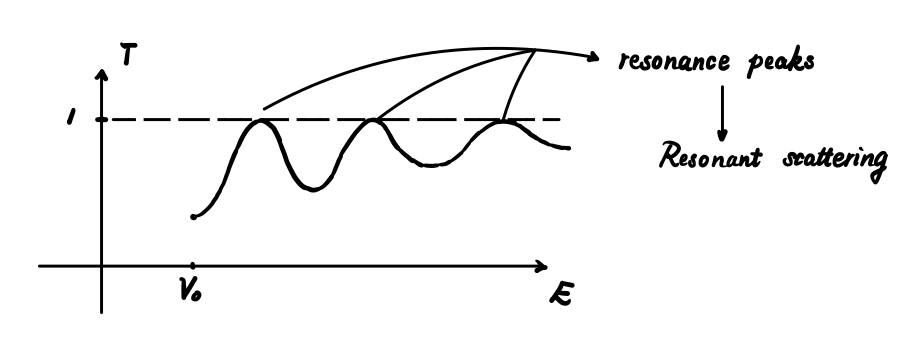
\includegraphics[scale = 1]{square-barrier-transmission.png}
\end{center}
We may use this property to determine the thickness $a$ and potential $V_0$ from fitting this model to experimental data. This allows ``quantum sensing'' of a material. Since the condition for peaks in $T$ is $la = n\pi$, we have
\begin{align*}
    n\pi &= a \cdot \sqrt{\frac{2\mu(E - V_0)}{\hbar^2}} \\
    E - V_0 &= \frac{n^2 \pi^2}{a^2} \cdot \frac{\hbar^2}{2\mu}
\end{align*}
which gives us the energy of a particle in a box of size $a$. The resonant peaks occur where $a$ is a half-integer multiple of the particle's wavelength. And not passing the barrier is the same as wavelength misalignment.

\subsection{Quantum Tunnelling - 量子隧穿}
Similar to the square barrier, the ansatz of quantum tunnelling will be:
$$\psi(x) = \begin{cases}
    Ae^{\imag k x} + Be^{-\imag k x}, & L, k = \sqrt{\frac{2\mu E}{\hbar^2}} \\
    Ce^{b x} + De^{-b x}, & \text{interaction, } b = \sqrt{\frac{2\mu(V_0 - E)}{\hbar^2}} \\
    Fe^{\imag k x}, & R, k = \sqrt{\frac{2\mu E}{\hbar^2}}
\end{cases}$$
From \href{https://en.wikipedia.org/wiki/Quantum_tunnelling}{\textcolor{cyan}{Wikipedia}}, the graphical representation of quantum tunnelling is the following:
\begin{center}
    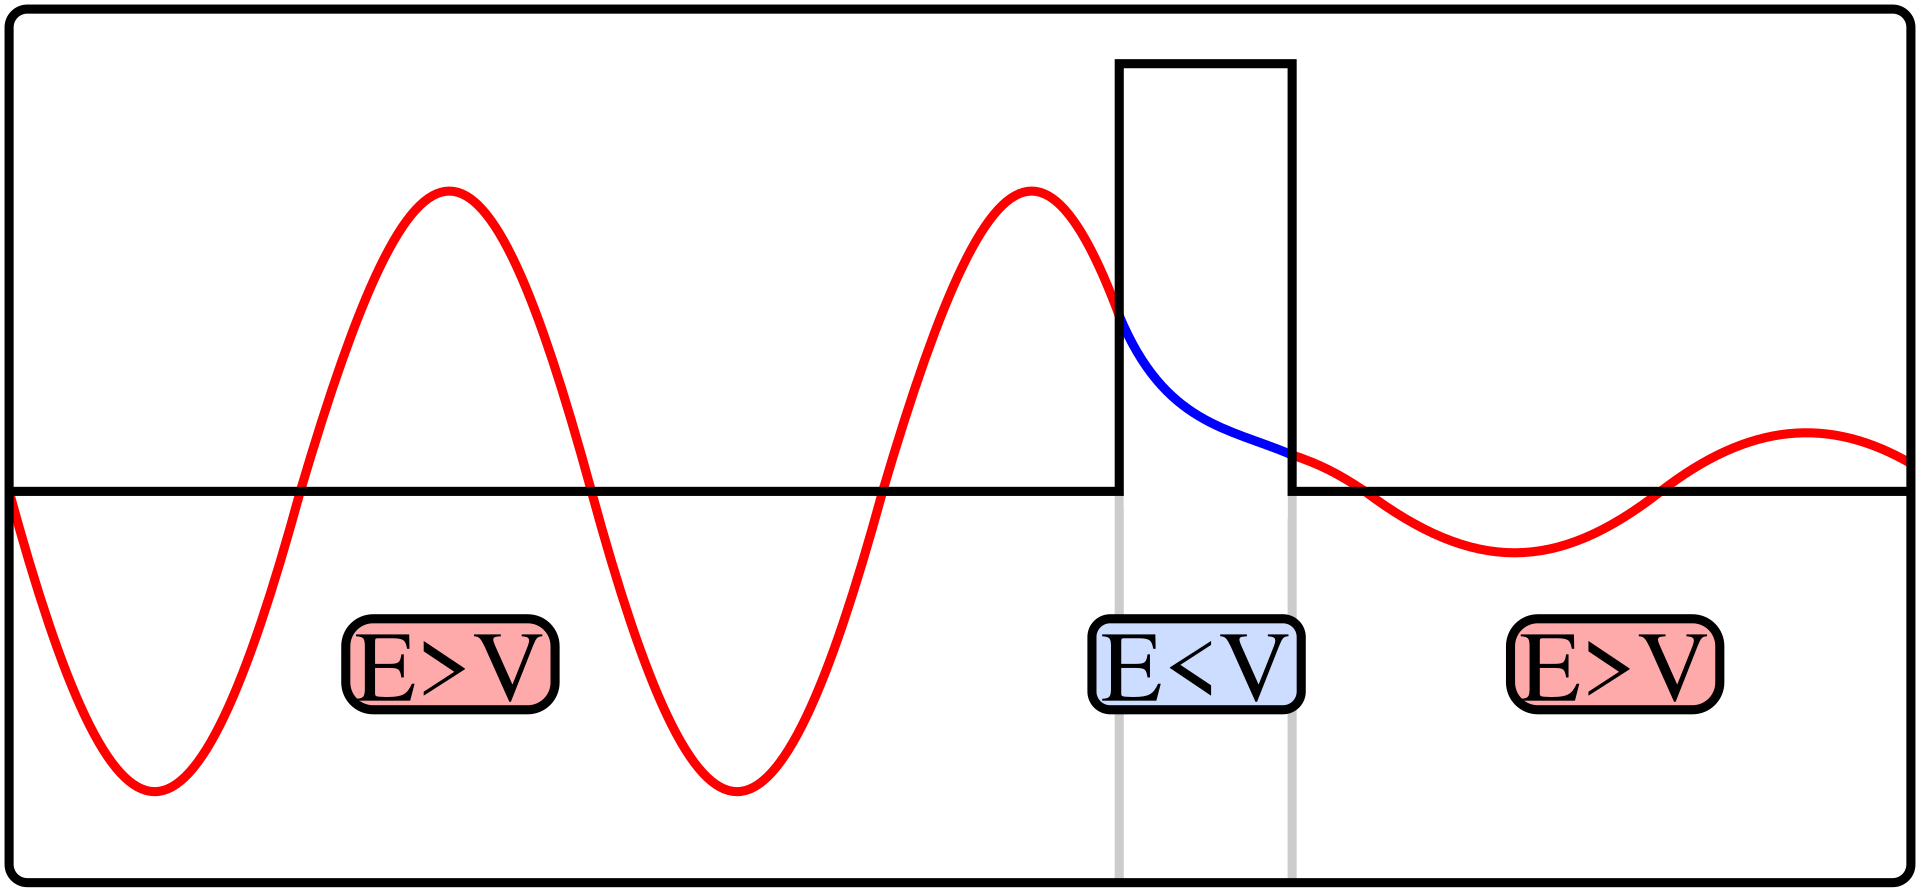
\includegraphics[scale = 0.2]{quantum-tunnelling.png}
\end{center}
That is, there exists a possibility to find the particle on the other side of the box, but the amplitude is drastically dampened.

\newpage